\subsection{Integrali doppi su domini rettangolari}

\subsubsection{Integrali di una funzione limitata definita su un rettangolo}

Per calcolare l'area del sottografico di una funzione in due variabili arriveremo alla definizione di integrale iniziando dal cercare l'area di un rettangolo suddiviso in più rettangoli; come fatto per gli integrali a una variabile.

Sia \(R \in \R^2\) un rettangolo chiuso \(R = [a,b]\times [c,d]\):

\[
    R = \{(x,y) \in \R^2 \giventhat a \le x \le b, c \le y \le d \}
\]

\(D_1\) suddivisione di \([a,b]\), \(D_2\) suddivisione di \([c,d]\).

\(D_1 \{x_0,x_1,\ldots,x_n\} \) con \(a = x_0 < x_1 < \cdots < x_n = b\) (\(n+1\) punti ordinati)

\(D_2 \{y_0,y_1,\ldots,y_n\} \) con \(c = y_0 < y_1 < \cdots < y_n = d\) (\(n+1\) punti ordinati)


\(D = D_1 \times D_2\) suddivisione di \(R\) in più rettangoli.

\([a,b]\) è suddiviso in \(n\) intervalli \([x_{i-1}, x_i]\) con \(i = 1 \ldots n\)

\([c,d]\) è suddiviso in \(m\) intervalli \([y_{j-1}, y_j]\) con \(j = 1 \ldots m\)

\(R\) è suddiviso in \(n\cdot m\) rettangoli \(R_{ij} = [x_{i-1}, x_i] \times [y_{j-1}, y_j]\):

\[
    R_{ij} = \{(x,y) \in \R^2 \giventhat x_{i-1} \le x \le x_i,\ y_{j-1} \le  y \le y_j\}
\]

L'area di uno dei rettangoli è: \(A_{ij} = A(R_{ij}) = (x_i - x_{i-1}) \cdot (y_j - y_{j-1})\)

\filbreak{}
\subsubsection{Somma superiore e somma inferiore}

Supponiamo \(f: R \to \R \) limitata, dunque \(\exists m,M \giventhat m \le f(x,y) \le M ~\forall (x,y) \in R\).

Se consideriamo la suddivisione in più rettangoli, per \(i=1 \cdots n,\ j= 1 \cdots m\) abbiamo:

\[
    m_{ij} = \underset{R_{ij}}{\inf}\, f(x,y)
\]

\[
    M_{ij} = \underset{R_{ij}}{\sup}\, f(x,y)
\]

\defn{Somma inferiore}{
    Definiamo la somma inferiore di \(f\) rispetto a \(D\):

    \[
        s(f,D) = \sum^{n}_{i=1} \sum^{m}_{j=1} m_{ij} \cdot A_{ij}
    \]

    cioè la somma dei parallelepipedi che stanno sotto la funzione.
}

\defn{Somma superiore}{
    Definiamo la somma superiore di \(f\) rispetto a \(D\):

    \[
        S(f,D) = \sum^{n}_{i=1} \sum^{m}_{j=1} M_{ij} \cdot A_{ij}
    \]

    cioè la somma dei parallelepipedi che racchiudano la funzione.
}

Per ogni suddivisione \(D\) di \(R\) vale sempre:

\[
    m(b-a)(d-c) \le s(f,D) \le S(f,D) \le M(b-a)(d-c)
\]

dove, \((b-a)(d-c)\) è l'area di tutto il rettangolo \(R\).

Risultano dunque ben definite le quantità:

\[
    \underset{D}{\inf}\, S(f,D) \quad\text{e}\quad \underset{D}{\sup}\, s(f,D)
\]

quindi si può avere:

\begin{itemize}
    \item \(\sup s(f,D) < \inf S(f,D)\)
    \item \(\sup s(f,D) = \inf S(f,D)\) in questo caso \(f\) si dice \textbf{integrabile}
\end{itemize}

\filbreak{}
\subsubsection{Funzione integrabile secondo Riemann}

\defn{Funzione integrabile secondo Riemann}{ Sia \(f: R = [a,b] \times [c,d] \to \R \) limitata, si dice integrabile secondo Riemann se:

\[
    \sup s(f,D) = \inf S(f,D)
\]

In tal caso il valore comune si dice \textbf{integrale}  di \(f\) su \(R\) si indica in vari modi:

\[
    I(f,R)
    = \iint_R f
    = \iint_{R} f(x,y) \diff{x}\diff{y}
    = \int_{a}^{b} \int_{c}^{d} f(x,y) \diff{x}\diff{y}
\]
}

La \textbf{classe delle funzioni integrabili} secondo Riemann su \(R\) si indica \(\R(R)\).

\proposizione{Funzioni costanti}{
    Ogni funzione costante \(f(x,y) = K\) è integrabile su \(R\):

    \[
        \iint_R {K} \diff{x}\diff{y} = K(b-a) (d-c)
    \]
}

\teorema{Integrabilità funzioni limitate}{
Sia \(f: R \to \R \) limitata;

\(f \in \R(R) \iff \forall \varepsilon \), anche piccolissimo, esiste una suddivisione \(D_\varepsilon \) di \(R\) per cui:

\[
    S(f,D_{\varepsilon}) - s(f,D_{\varepsilon}) < \varepsilon
\]
}

\proposizione{Funzioni continue}{
    Sia \(f\) continua su \(R\);

    \(f\) è quindi limitata su \(R \implies \) \(f\) è integrabile su \(R\).
}

\vbox{
\subsubsection*{Esempio di funzione non integrabile secondo Riemann}

\(R = [0,1] \times [0,1]\):

\[
    f(x,y) = \begin{cases}
        1 & \text{se } (x,y) \in \mathbb{Q} \\
        0 & \text{altrimenti}
    \end{cases}
\]

\begin{align*}
     & s = \sum^{n}_{i=1} \sum^{m}_{j=1} 0 \cdot (x_i - x_{i-1})(y_j - y_{j-1}) = 0 (b-a) (d-c) = 0 (1-0)(1-0) = 0 \\
     & S = \sum^{n}_{i=1} \sum^{m}_{j=1} 1 \cdot (x_i - x_{i-1})(y_j - y_{j-1}) = 1 (b-a) (d-c) = 1 (1-0)(1-0) = 1
\end{align*}

Essendo \(s \neq S\) allora \(f\) non è integrabile
}

\filbreak{}
\subsubsection{Interpretazione Geometrica}

Nel caso unidimensionale l'integrale era l'area del sottografico (trapezoide). In due variabili è il valore di un solido detto \textbf{cilindroide}.

Sia \(f \in \R(R)\) e \(f \ge 0\).

Il suo integrale \(\iint_R f\) si può interpretare come volume di \(T\) solido in \(\R^{3}\) detto cilindroide, delimitato dal basso da \(R\) e dall'alto dal grafico di \(f\).

Nella seguente figura abbiamo \(s(f,R)\) a sinistra e \(S(f,R)\) a destra:

\begin{center}
    \begin{tabular}{c c c}
        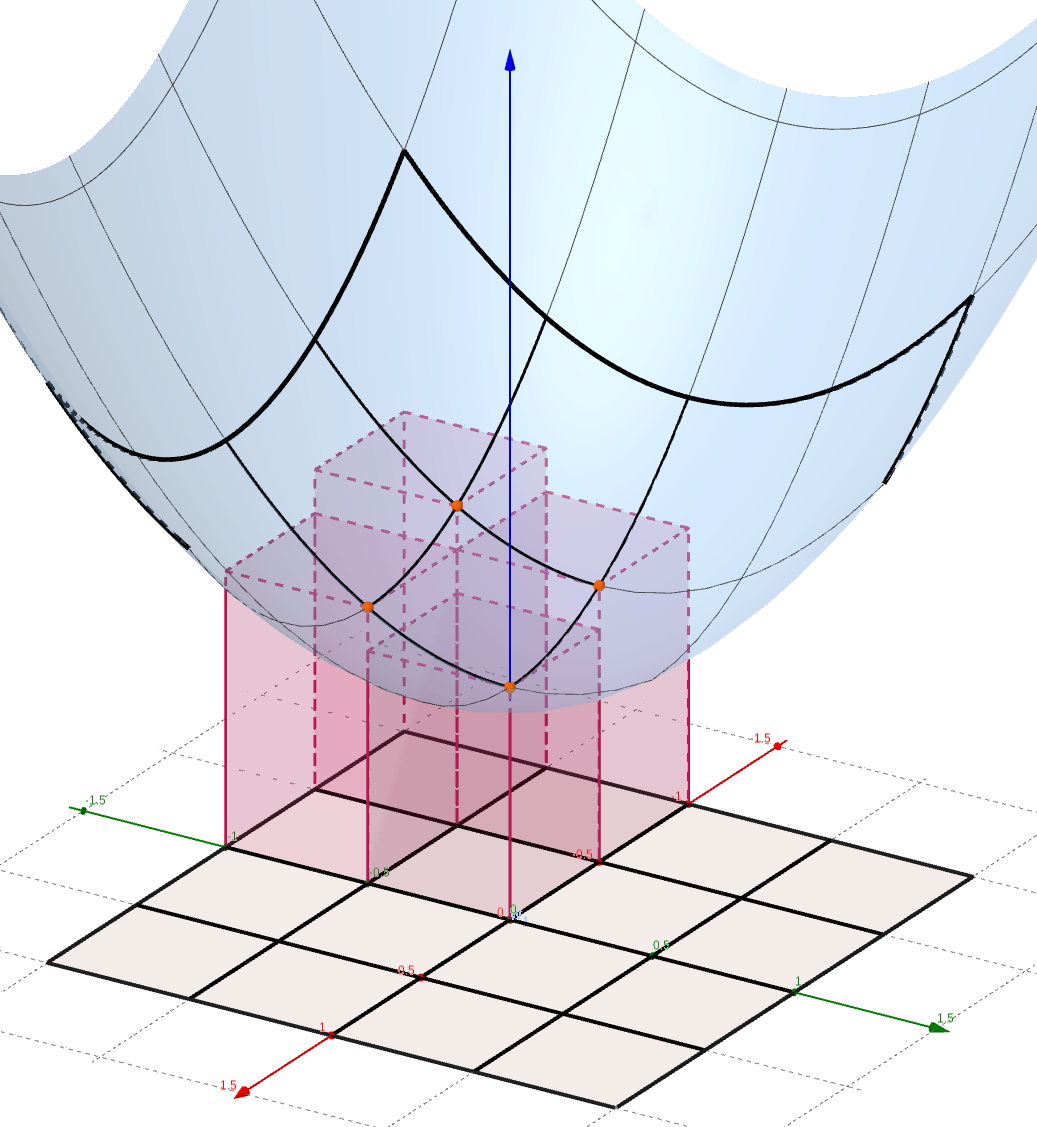
\includegraphics[width=0.45\textwidth]{integrali-doppi-rettangoli-min.png}
         &
        \hspace{3mm}
         &
        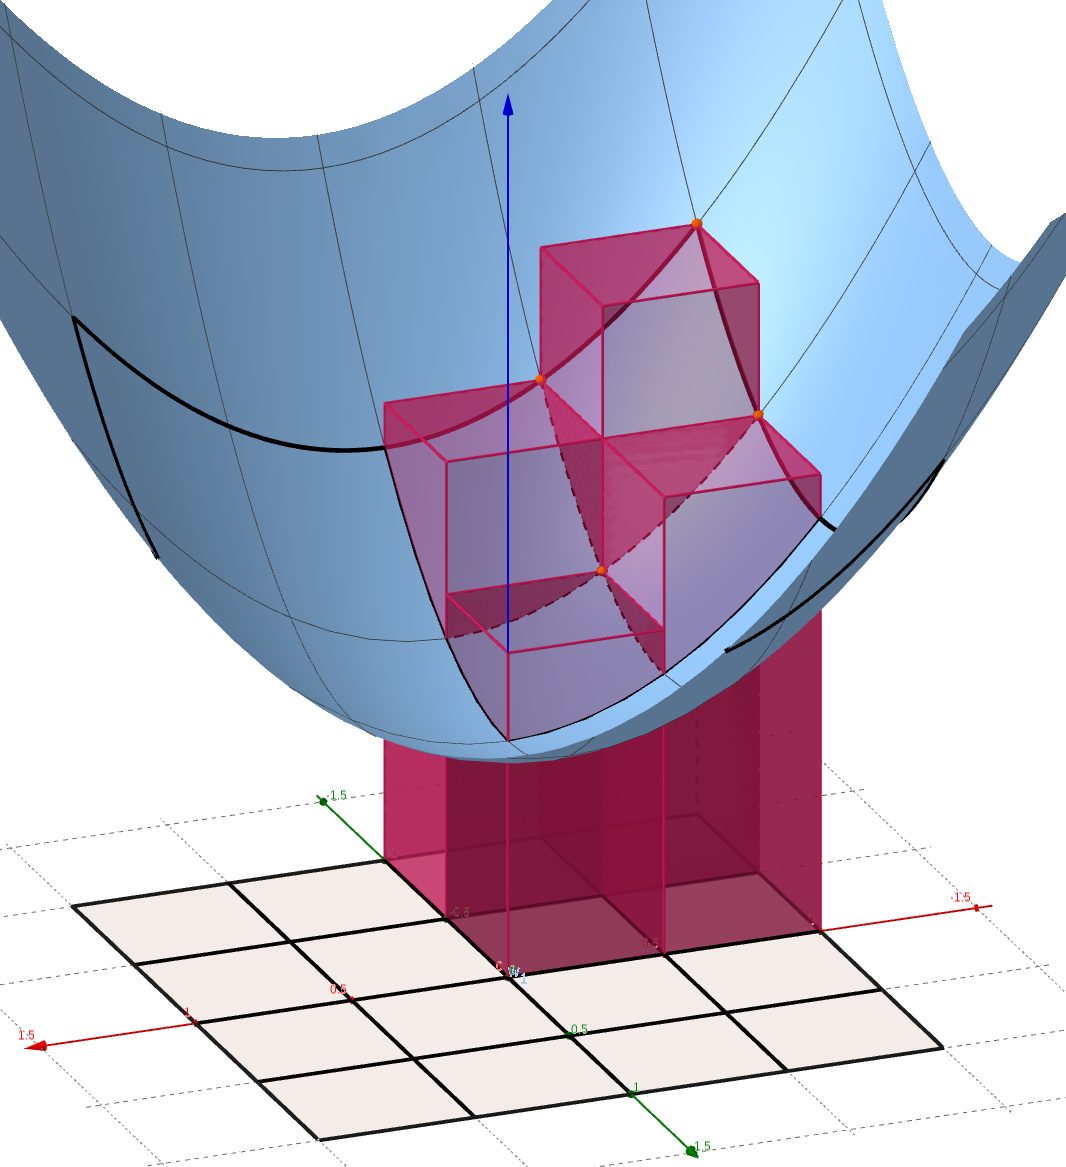
\includegraphics[width=0.45\textwidth]{integrali-doppi-rettangoli-max.png}
    \end{tabular}
\end{center}

Ogni addendo di \(s\) e \(S\) è un parallelepipedo (alto \(m_{ij}\) per \(s\) e basso \(M_{ij}\) per \(S\)).

Quindi \(s\) è il volume del solido \textbf{contenuto} in \(T\) e \(S\) il volume del solido \textbf{che contiene} \(T\).

Siccome l'integrale è \(\sup s = \inf S\) abbiamo che esso è proprio il volume di T.

\filbreak{}
\subsubsection{Calcolo degli integrali doppi su rettangoli}

Si fanno variare \(x\) e \(y\) separatamente, per ottenere due integrali semplici.

Integrare parzialmente rispetto a \(x\): considero le tracce di \(f\) con \(y\) fissato e integro rispetto a \(x\).

Integrare parzialmente rispetto a \(y\): considero le tracce di \(f\) con \(x\) fissato e integro rispetto a \(y\).

\teorema{di riduzione}{ Sia \(f \in \R(R)\) dove \(R=[a,b] \times [c,d]\)

\begin{enumerate}
    \item Se, per ogni \(y \in [c,d]\), esiste l'integrale:

          \[
              G(y) = \int_{a}^{b} f(x,y) \diff{x}
          \]

          allora la funzione \(y \to G(y)\) è integrabile in \([c,d]\) e vale la formula:

          \[
              \iint_R f = \int_{c}^{d} {G(y)} \diff{y} = \int_{c}^{d} {\left(\int_{a}^{b} f(x,y) \diff{x} \right) \diff{y}}
          \]

    \item Se, per ogni \(x \in [a,b]\) esiste l'integrale

          \[
              H(x) = \int_{c}^{d} f(x,y) \diff{x}\diff{y}
          \]

          allora la funzione \(x \to H(x)\) è integrabile in \([a,b]\) e vale la formula:

          \[
              \iint_R f = \int_{a}^{b} H(x) \diff{x} = \int_{a}^{b} {\left(\int_{c}^{d} f(x,y) \diff{y} \right) \diff{x}}
          \]

\end{enumerate}
}

Chiaramente, se la \(f\) è continua in \(R\) allora questo teorema vale poiché la funzione è integrabile.

\teorema{Formule di riduzione}{
Sia \(R=[a,b]\times [c,d]\);

Sia \(f: R \to \R \) \underline{continua};

Se questo è vero, allora \(f \in R(\R) \) e si ha:

\[
    \iint_R f(x,y) \diff{x}\diff{y} = \int_{a}^{b} {\left(\int_{c}^{d} f(x,y) \diff{y} \right)} \diff{x} = \int_{c}^{d} {\left(\int_{a}^{b} f(x,y) \diff{x} \right) \diff{y}}
\]
}

\filbreak{}
\subsubsection*{Esempio}

Sia \(f(x,y)= x^{-3} e^{\frac{y}{x}}\) dove \(R = [1,3] \times [0,1]\)

\(f\) è continua in \(R\) e dunque possiamo usare la formula:

\[
    \iint_R f(x,y) \diff{x}\diff{y} = \iint_R {x ^{-3} e ^{ \frac{y}{x}}} \diff{x}\diff{y}
\]
\[
    \int_{a}^{b} {\left(\int_{c}^{d} f(x,y) \diff{y} \right)} \diff{x} = \int_{1}^{3} {\left(\int_{0}^{1} {x ^{-3} e ^{ \frac{y}{x}}} \diff{y} \right) \diff{x}}
\]

prima facciamo:

\[
    \int_{0}^{1} x ^{-3} e ^{ \frac{y}{x}} \diff{y} =
    x ^{-3} \int_{0}^{1} e ^{ \frac{y}{x}} \diff{y} =
    x ^{-3} \Eval{\left[ x e ^{ \frac{y}{x}} \right]}{0}{1} =
    x ^{-3} \left[ x e ^{ \frac{1}{x}}-x \right] =
    x ^{-2} \left(e ^{ \frac{1}{x}} -1\right)
\]

e dunque:

\begin{align*}
    \int_{1}^{3} x ^{-2} \left(e^{x^{-1}}-1\right) \diff{x} & = \int_{1}^{3} x ^{-2} e^{x^{-1}} \diff{x} + \int_{1}^{3} -x^{-2} \diff{x}    \\
                                                            & = - \int_{1}^{3} -x ^{-2} e ^{ \frac{1}{x}} \diff{x} - \int_{1}^{3} x^{-2}    \\
                                                            & = - \int_{1}^{3} e^t \diff{t} - \int_{1}^{3} x^{-2} \diff{x}                  \\
                                                            & = -\Eval{\left[ e^{x^{-1}}\right]}{1}{3} -\Eval{\left[ -x^{-1} \right]}{1}{3} \\
                                                            & = -\left( e ^{ \frac{1}{3}} - e \right) -\left[ -\frac{1}{3} - (-1) \right]   \\
                                                            & = -e ^{\frac{1}{3}} + e -\frac{2}{3}
\end{align*}
